\documentclass{article}


% if you need to pass options to natbib, use, e.g.:
%     \PassOptionsToPackage{numbers, compress}{natbib}
% before loading neurips_2023


% ready for submission
\usepackage[final, nonatbib]{neurips_2023}


% to compile a preprint version, e.g., for submission to arXiv, add add the
% [preprint] option:
%     \usepackage[preprint]{neurips_2023}


% to compile a camera-ready version, add the [final] option, e.g.:
%     \usepackage[final]{neurips_2023}


% to avoid loading the natbib package, add option nonatbib:
%    \usepackage[nonatbib]{neurips_2023}


\usepackage[utf8]{inputenc} % allow utf-8 input
\usepackage[T1]{fontenc}    % use 8-bit T1 fonts
\usepackage{hyperref}       % hyperlinks
\usepackage{url}            % simple URL typesetting
\usepackage{booktabs}       % professional-quality tables
\usepackage{amsfonts}       % blackboard math symbols
\usepackage{nicefrac}       % compact symbols for 1/2, etc.
\usepackage{microtype}      % microtypography
\usepackage{xcolor}         % colors

\usepackage[spanish, es-tabla]{babel}

\usepackage[pdftex]{graphicx}
\usepackage{pgf}
\usepackage{subcaption}
\graphicspath{{./fg/}}



%% biblatex
\usepackage[style = numeric, backend = biber, sorting = none, doi = false, isbn = false, url = true]{biblatex}
% \usepackage[defernumbers = true, style = numeric, backend = biber, sorting = none, doi = false, isbn = false, url = true]{biblatex}
% \usepackage[style = numeric, backend = biber, sorting = none]{biblatex}    % REFERENCIAS como section
\AtEveryBibitem{
    \clearfield{urlyear}
    \clearfield{urlmonth}
} % Do not show the "(visited on <date>)" on the references
\DefineBibliographyStrings{spanish}{}
\usepackage{csquotes}
\addbibresource{./dmcyt.bib}
\renewcommand*{\bibfont}{\fontsize{9}{12}\selectfont}



\title{TP2: Redes en el cerebro}

\author{
  Víctor A.~Bettachini\\
  \texttt{bettachini@gmail.com}
  \And Vanesa Flores\\
  \texttt{vanesaflores0894@gmail.com}
  \And Tomás Gianni\\
  \texttt{tomasgianni11@gmail.com}
  \And Malena Pirola\\
  \texttt{malenapirola@gmail.com}\\
}


\begin{document}


\maketitle


% \begin{abstract}
%?
%\end{abstract}


% Enunciado
% Se sugiere realizar la entrega en formato latex, pero en este caso va a ser optativo (en el TP ya es obligatorio, sugerimos que lo usen de práctica). Pueden acceder a formatos de distintas conferencias a través de Overleaf, en particular les sugerimos el formato de NeurIPS que es una de las conferencias más importantes en IA.
% Se sugiere un máx de 4 carillas (mín 2), no se debe incluir código a menos que sea algo esencial que hayan desarrollado ustedes (es preferible en este caso incluir el pseudo-código). Aclaración: No vamos a corregir código en la entrega.
% El pre TP es individual.


% \section{Introducción}

\section{Materiales y métodos}

\paragraph{Datos}
Se hace uso de datos producto de la medición de la señal de resonancia magnética funcional (fMRI).
Definidos 116 volúmenes de interés del cerebro en términos de su activación \cite{tzourio-mazoyer_automated_2002}, se publicaron coeficientes de correlación lineal entre sus medias en distintos segmentos temporales \cite{tagliazucchi_large-scale_2013}.
Con estos datos se generó una matriz de correlación, y a partir de la misma los grafos analizados en este trabajo.


\paragraph{Recurso informático} 
Un cuaderno (notebook) Jupyter provisto por los docentes en el sitio web denominado ``Campus'' \cite{kamienkowski_curso_2023} es la plantilla donde se escribió código en lenguaje Python.
Este explotó funciones de las biblioteca NetworkX \cite{hagberg_exploring_2008}.



\subsection{Preprocesamiento de los datos}
% Cada actividad realizada se describe bajo los titulos que figuran en el enunciado del trabajo práctico publicado en el

\paragraph{Carga del conjunto de datos} 
Los archivos provistos corresponden a los estadíos de sueño N1, N2, N3 y al estado despierto W para 18 sujetos.
Estos estuvieron acompañados de una tabla que describe la denominación y  ubicación espacial las regiones en que se parcializó el cerebro.


\section{Resultados}

\subsection{Tarea 1: Visualización}

\paragraph*{Promedio de correlaciones}
Tras calcular el promedio de correlaciones de todos los sujetos para cada estadio del sueño, se obtuvieron las matrices de adyacencia que se muestran en la figura \ref{fg:matrizAdyacenciaEstadoSueño}.

\begin{figure}[ht]
  \centering
  \includegraphics[width= \linewidth]{matrizAdyacenciaEstadoSueño.png}
  \caption{Matrices de adyacencia del promedio de las correlaciones de activación de volúmenes cerebrales en el estado despierto, W, y los tres estadíos de sueño. La numeración de los volúmenes es la utilizada en \cite{tzourio-mazoyer_automated_2002}.
	}
	\label{fg:matrizAdyacenciaEstadoSueño}
\end{figure}


\paragraph*{Tamaño de la componente gigante} 
El número de nodos de la componente gigante de cada grafo se muestra en la figura \ref{fg:númeroNodosComponenteGigante}.

\begin{figure}[ht]
  \centering
  \includegraphics[width= 0.8\linewidth]{númeroNodosComponenteGigante.png}
  \caption{Número de nodos de la componente gigante de los grafos de los cuatro estados de sueño y el estado despierto.
	}
	\label{fg:númeroNodosComponenteGigante}
\end{figure}

Una inspección visual revela los siguientes saltos

\begin{table}[ht]
	\centering
\begin{tabular}{ccc}
	\toprule
	Estado de sueño & $\delta$  & $\Delta$ nodos \\
	\midrule
	W & $\approx 0.055$ &  $\approx 75 \rightarrow \approx 95$ \\
	N1 & $\approx 0.065$ &  $\approx 75 \rightarrow \approx 95$ \\
	N2 & $\approx 0.095$ &  $\approx 80 \rightarrow \approx 105$ \\
	N3 & $\approx 0.03$ &  $\approx 65 \rightarrow \approx 90$ \\
	\bottomrule
\end{tabular}
\bigskip
\caption{Saltos en el tamaño de la componente gigante.}
\label{tb:saltos}
\end{table}

Pendientes:\\
Interpretar las curvas\\
¿Qué indican los saltos?


\paragraph{Análisis de un salto}
%La figura \ref{fg:saltoN2} ilustra el salto en el tamaño de la componente gigante en el promedio para los participantes del estudio en el estadío de sueño N2 que se produce en la vecindad de una $\delta = 0.095$.
%
%\begin{figure}[ht]
%	\centering
%	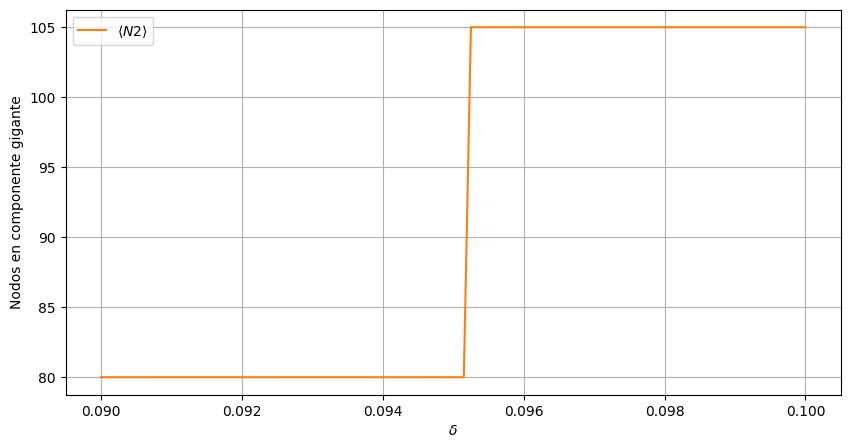
\includegraphics[width= 0.8\linewidth]{saltoN2.png}
%	\caption{Detalle del salto en el número de nodos del promedio para el estado de sueño N2 en torno a $\delta = 0.095$.
%	}
%	\label{fg:saltoN2}
%\end{figure}

Para el salto que se produce para el estado de sueño N2 en la vecindad de una $\delta = 0.095$, se muestra en la figura \ref{fg:grafoSaltoN2} el grafo de las correlaciones previo y a posteriori.

\begin{figure}[ht]
	\centering
	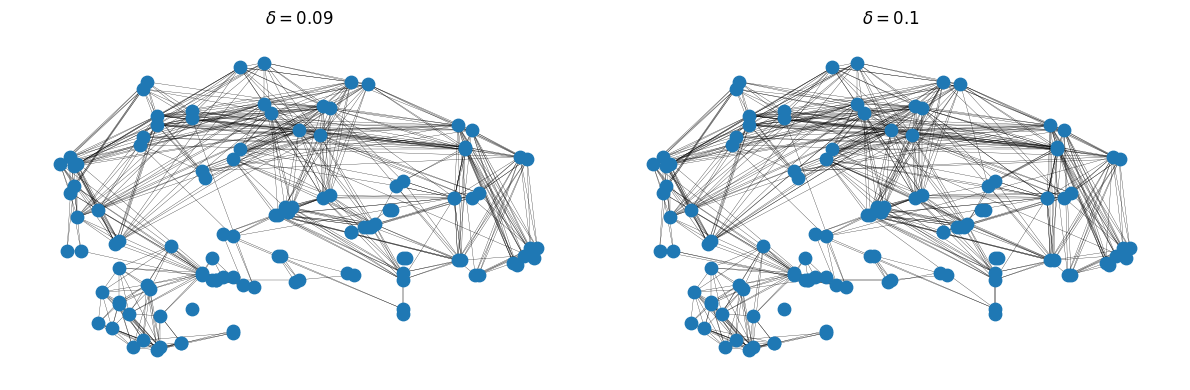
\includegraphics[width= \linewidth]{grafoSaltoN2.png}
	\caption{Grafo de las correlaciones previo y a posteriori del salto en el número de nodos del promedio para el estado de sueño N2 en torno a $\delta = 0.095$.
	}
	\label{fg:grafoSaltoN2}
\end{figure}


\paragraph*{Variación del grado promedio}

La figura \ref{fg:gradoPromedio} muestra una relación lineal entre el grado promedio, $\langle k \rangle$, de los grafos de los cuatro estados de sueño y el estado despierto.
Esto es lógico pues la definición de densidad se da en función de la cantidad de enlaces que hay en la red, por lo que a mayor densidad, mayor cantidad de enlaces y por lo tanto mayor grado promedio.
La expresión que las relaciona es $\delta = \frac{2L}{N(N-1)}$, donde $p$ es la densidad, $L$ es la cantidad de enlaces y $N$ es la cantidad de nodos. Si despejamos $L$ de esta expresión y la reemplazamos en la expresión de grado promedio, obtenemos que $\langle k \rangle = \frac{2 \delta (N-1)}{N}$, que es una función lineal de $\delta$.

\begin{figure}[ht]
	\centering
	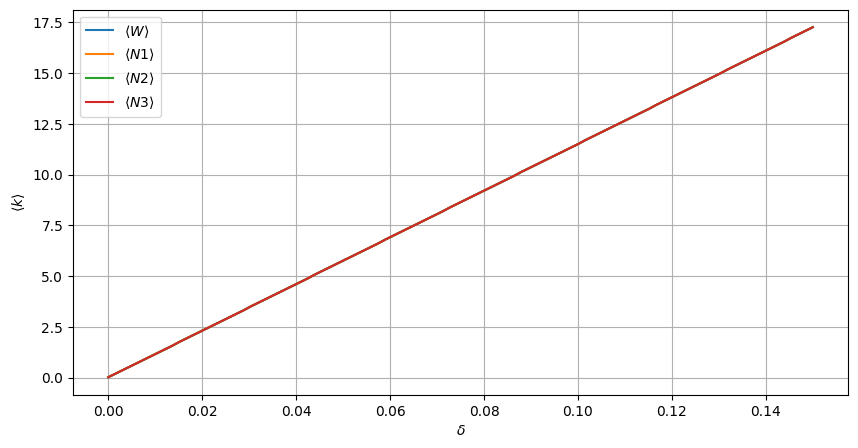
\includegraphics[width= 0.8\linewidth]{gradoPromedio.png}
	\caption{Grado promedio de los grafos de los cuatro estados de sueño y el estado despierto.
	}
	\label{fg:gradoPromedio}
\end{figure}


\paragraph*{Coeficiente de clustering promedio}

La figura \ref{fg:coeficienteClusteringPromedio} muestra una relación lineal entre el coeficiente de clustering promedio, $\langle C \rangle$, de los grafos de los cuatro estados de sueño y el estado despierto.

\begin{figure}[ht]
	\centering
	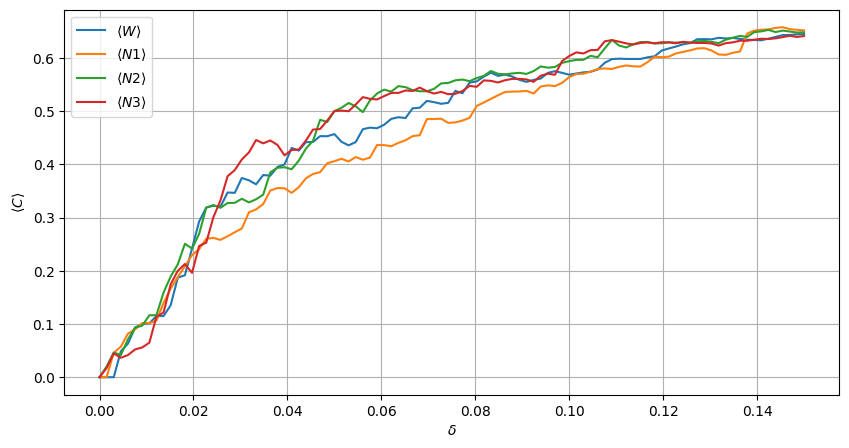
\includegraphics[width= 0.8\linewidth]{coeficienteClusteringPromedio.png}
	\caption{Coeficiente de clustering promedio de los grafos de los cuatro estados de sueño y el estado despierto.
	}
	\label{fg:coeficienteClusteringPromedio}
\end{figure}


\paragraph*{Eficiencia global}

La figura \ref{fg:eficienciaGlobal} muestra una relación lineal entre la eficiencia global de los grafos de los cuatro estados de sueño y el estado despierto.

\begin{figure}[ht]
	\centering
	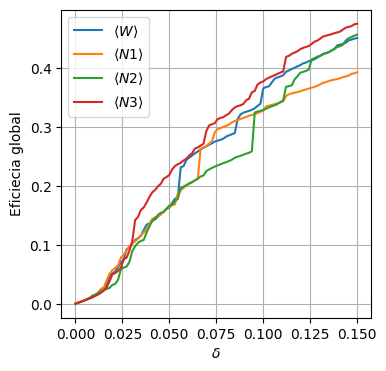
\includegraphics[width= 0.8\linewidth]{eficienciaGlobal.png}
	\caption{Eficiencia global de los grafos de los cuatro estados de sueño y el estado despierto.
	}
	\label{fg:eficienciaGlobal}
\end{figure}


\paragraph*{Centralidad de autovector}

La figura \ref{fg:centralidadAutovector} muestra una relación lineal entre la centralidad de autovector de los grafos de los cuatro estados de sueño y el estado despierto.

\begin{figure}[ht]
	\centering
	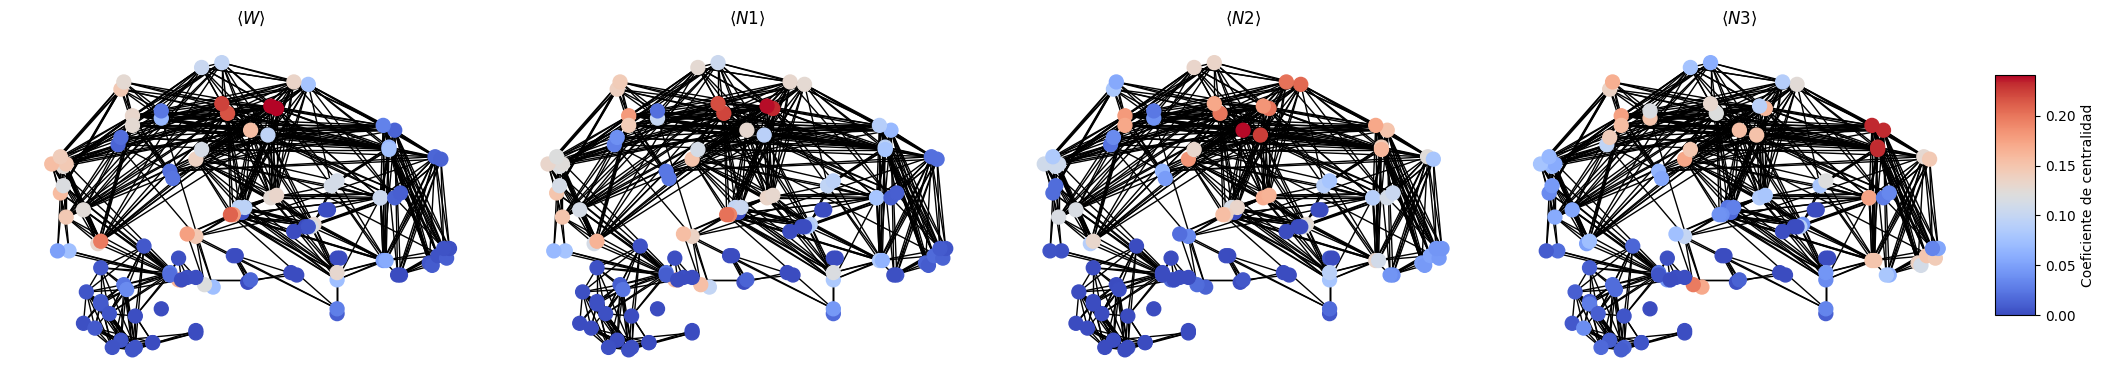
\includegraphics[width= \linewidth]{centralidadDensidadCeroPuntoDoce.png}
	\caption{Centralidad de autovector de los grafos de los cuatro estados de sueño y el estado despierto.
	}
	\label{fg:centralidadAutovector}
\end{figure}


\subsection{Tarea 2: Comunidades y coeficiente de modularidad}

\paragraph*{Coeficiente de modularidad en función de $\delta$}

La figura \ref{fg:coeficienteModularidad} muestra una relación lineal entre el coeficiente de modularidad de los grafos de los cuatro estados de sueño y el estado despierto.

\begin{figure}[ht]
	\centering
	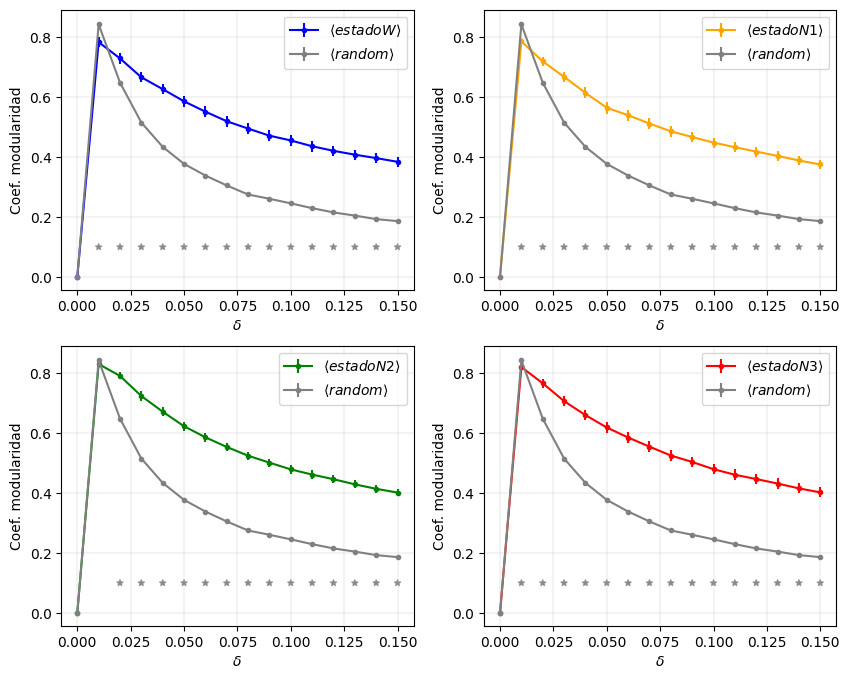
\includegraphics[width= 0.8\linewidth]{coeficienteModularidad.png}
	\caption{Coeficiente de modularidad en función de $\delta$ para los grafos de los cuatro estados de sueño y el estado despierto.
	}
	\label{fg:coeficienteModularidad}
\end{figure}


\paragraph*{Variación de cantidad de comunidades con $\delta$}

La figura \ref{fg:cantidadComunidades} muestra una relación lineal entre la cantidad de comunidades de los grafos de los cuatro estados de sueño y el estado despierto.

\begin{figure}[ht]
	\centering
	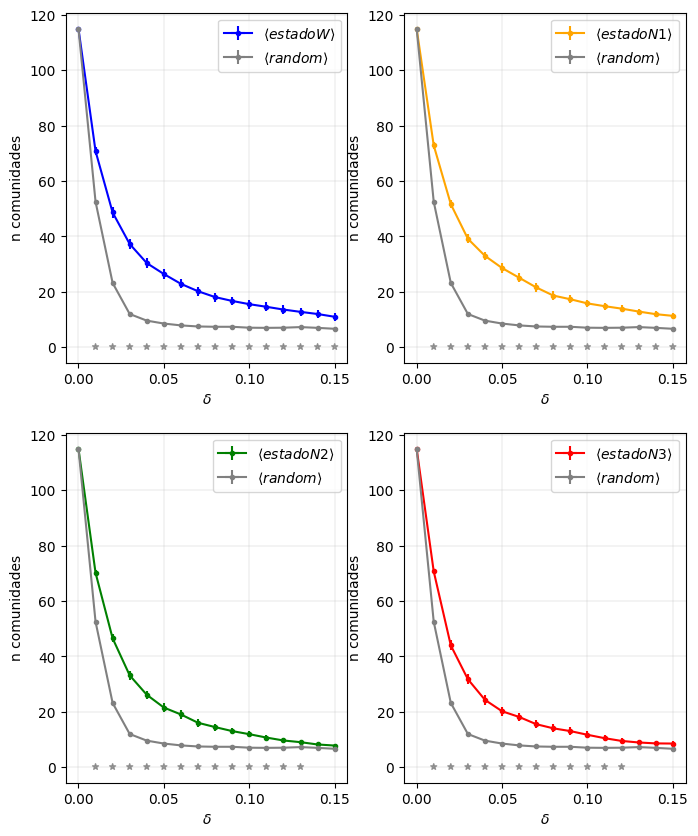
\includegraphics[width= 0.8\linewidth]{cantidadComunidades.png}
	\caption{Cantidad de comunidades en función de $\delta$ para los grafos de los cuatro estados de sueño y el estado despierto.
	}
	\label{fg:cantidadComunidades}
\end{figure}


% \section{Discusión y conclusiones}

\printbibliography[title= Referencias, heading=bibintoc]

\end{document}
